¿Cuál es el área del triángulo rectángulo de la figura \ref{fig:area_rectangulo_02}?

\begin{figure}[H]
    \begin{center}
        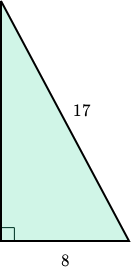
\includegraphics[width=0.15\linewidth]{../images/area_rectangulo_02.png}
    \end{center}
    \caption{}
    \label{fig:area_rectangulo_02}
\end{figure}
\begin{solutionbox}{13cm}

    \begin{minipage}{0.6\textwidth}
        Para determinar el área del triángulo debemos saber la base y la altura. Llamemos $x$ a la longitud (ver Figura \ref{fig:area_rectangulo_02a}).
        Cuando tenemos un triángulo rectángulo, podemos usar el teorema de Pitágoras para obtener la longitud del cateto.
        La ecuación para el teorema de Pitágoras es:
        \[c^2=a^2+b^2\]
        En este caso, $a=8$, $b=x$ y $c=17$, Entonces,
        \begin{align*}
            8^2+x^2 & =17^2   \\
            64+x^2  & =289    \\
            x^2     & =289-64 \\
            x^2     & =225    \\
            x       & =15
        \end{align*}
        La altura del triángulo es 15. El área del triángulo es:

        \begin{align*}
            A & =\frac{1}{2}bx              \\
            A & =\frac{1}{2}\cdot 8\cdot 15 \\
            A & =60 \text{ u}^2
        \end{align*}
    \end{minipage}\hfill
    \begin{minipage}{0.35\textwidth}
        \begin{figure}[H]
            \centering
            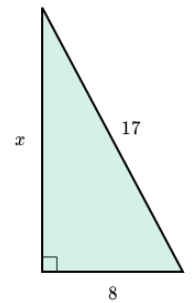
\includegraphics[width=0.5\linewidth]{../images/area_rectangulo_02a.png}
            \caption{}
            \label{fig:area_rectangulo_02a}
        \end{figure}
    \end{minipage}
\end{solutionbox}
